\documentclass[11pt]{article}

\usepackage[T1]{fontenc}
\usepackage[utf8]{inputenc}
\usepackage[margin=1in]{geometry}
\usepackage{graphicx}
\usepackage{booktabs}
\usepackage{amsmath}
\usepackage{amssymb}
\usepackage{newtxtext}
\usepackage{newtxmath}
\usepackage{microtype}
\usepackage{caption}
\usepackage{titlesec}
\usepackage{natbib}
\usepackage{xcolor}
\usepackage[hidelinks]{hyperref}

\graphicspath{{figures/}}
\captionsetup{font=small,labelfont=bf,labelsep=period}
\setlength{\parindent}{1.4em}

% tighter, more journal-like section headings
\titleformat{\section}{\normalfont\large\bfseries}{\thesection}{0.6em}{}
\titleformat{\subsection}{\normalfont\normalsize\bfseries}{\thesubsection}{0.6em}{}
\titlespacing*{\section}{0pt}{1.5ex plus .3ex minus .2ex}{0.9ex}
\titlespacing*{\subsection}{0pt}{1.2ex plus .2ex}{0.6ex}

% keep the bibliography compact so it does not strand a near-empty final page
\setlength{\bibsep}{0.2ex plus 0.2ex}

% tighten whitespace around floats for a more compact, journal-like vertical rhythm
\setlength{\textfloatsep}{13pt plus 2pt minus 2pt}
\setlength{\intextsep}{11pt plus 2pt minus 2pt}

\title{\textbf{Multimodal Cancer-Cell Classification under Patient Shift:\\
A Distillation-Based Recipe for Small-$N$ Microscopy}}
\author{Rafael Tavares Proen\c{c}a\\[2pt]
{\small 1MD042 --- Advanced Deep Learning for Image Processing}\\
{\small Uppsala University, Spring 2026}}
\date{}

\begin{document}
\maketitle

\begin{abstract}
\noindent
On this dataset, classifying oral-cancer cells from paired brightfield (BF) and fluorescence (FL)
microscopy is a small-$N$, out-of-distribution problem: only 12 patients are available for training,
and every test cell comes from a patient the model has never seen. I argue, and show empirically,
that in this regime the dominant lever is the size of the \emph{effective} labelled set --- not model
capacity or regularisation. Starting from a dual-branch EfficientNet-B0 with a shift-aware training
recipe (adaptive batch normalisation, test-set stain normalisation, a per-patient multiple-instance
loss, and heavy paired augmentation), I grow the training signal by treating the unlabelled test
images as extra supervision: first with hard pseudo-labels \citep{lee2013}, then with soft-target
knowledge distillation \citep{hinton2015}. Across the full recipe the public-leaderboard AUC rises from
$0.7455$ to $0.8236$ (a cumulative $+0.078$); the soft-distillation step alone --- the teacher's raw
probabilities on all $59{,}040$ test cells used as targets --- contributes $+0.042$ of that, the largest
single jump and roughly four standard errors above the seed-to-seed noise floor. I also document what
did \emph{not} work, namely cross-modal self-supervised pre-training,
same-domain architecture transfer, stacking unvalidated changes, and cross-recipe ensembling,
because each failure diagnosed a property of the data that directly shaped the final recipe.
\end{abstract}

\noindent\textbf{Keywords:} semi-supervised learning; knowledge distillation; pseudo-labelling; domain
shift; multimodal microscopy; test-time adaptation; small-sample learning.

\section{Introduction}

The task is per-cell binary classification: given two co-registered $128\times128$ grayscale images of a
single cell (one brightfield, one fluorescence), predict whether the cell comes from a cancer patient.
Labels are supplied at the \emph{patient} level, so every cell inherits its patient's diagnosis,
and performance is scored by area under the ROC curve (AUC) on a held-out test set.

The defining feature of the dataset is its structure rather than its size. There are $\sim\!114{,}000$
labelled training cells, which sounds ample, but they come from only \textbf{12 patients}; the test
cells belong to entirely \emph{different} patients. With so few independent units, the central risk is
not under-fitting but learning the wrong invariance: a model that latches onto ``which patient is this''
instead of ``is this cancer'' can look excellent in cross-validation and then collapse on a
patient-disjoint test set. Every design decision in this project is, at bottom, an attempt to suppress
that patient shortcut and to make the most of a small labelled set.

This report presents the recipe that reached a public-leaderboard AUC of $0.8236$, the experiments that
led there, and, equally important for the methodology, the diagnosed failures along the way.

\section{Related work}

The recipe combines established ideas rather than introducing a new architecture, so it is best
understood through the lines of work it draws on.

\textbf{Learning from unlabelled data.} When labels are scarce but inputs are plentiful, two classic
strategies turn predictions into supervision. Pseudo-labelling \citep{lee2013} assigns hard labels to
confident unlabelled examples and trains on them as ground truth. Knowledge distillation
\citep{hinton2015}, building on earlier model compression \citep{bucila2006}, instead transfers a
teacher's full output distribution to a student, so the soft target carries the teacher's uncertainty
rather than a thresholded decision. I apply both to the unlabelled test images and find the soft variant
decisively better, consistent with the view that the discarded probability mass is where the extra
signal lives.

\textbf{Adapting to distribution shift.} Because the test patients differ from the training patients, the
train and test pixel statistics genuinely diverge. Adaptive batch normalisation \citep{li2016} addresses
this without labels by recomputing batch-norm statistics on the target data --- a cheap form of test-time
adaptation that I pair with test-set stain normalisation.

\textbf{Stable training and efficient backbones.} Stochastic weight averaging \citep{izmailov2018}
reduces run-to-run variance by averaging weights along the training trajectory, which matters when the
small patient count makes single runs noisy. For the backbone I use EfficientNet-B0 \citep{tan2019};
on twelve patients its small parameter count is an asset, since extra capacity mainly buys room to
memorise patient identity. The contribution here is not any single component but the finding that, in a
small-$N$ patient-shifted regime, enlarging the effective labelled set with soft distillation dominates
the capacity and regularisation choices a larger-data setting would reward.

\section{Data and problem setting}

\begin{itemize}
  \item \textbf{Modalities.} Each cell has a paired BF and FL image at $128\times128$, grayscale.
  \item \textbf{Train.} $\sim\!114{,}302$ cells from $12$ patients ($\sim\!10$k cells/patient);
        $38.8\%$ are cancer-positive.
  \item \textbf{Test.} $59{,}040$ cells from patients \emph{disjoint} from training. The leaderboard is
        split into a public and a private portion.
  \item \textbf{Labels.} Patient-level (weak): a cell is labelled by its patient's diagnosis, so
        within-patient label noise is expected.
  \item \textbf{Metric.} AUC.
\end{itemize}

The patient-disjoint split is the central difficulty. Because brightness, staining and morphology vary more
\emph{between} patients than between classes, any representation that encodes patient identity will
generalise poorly. Two concrete consequences recur throughout: (i) cross-validation that does not group
by patient is dangerously optimistic, and (ii) the train and test pixel statistics genuinely differ
(the FL test images run roughly $20\%$ brighter), so na\"ive normalisation hurts.

\section{Method}

\subsection{Backbone selection: the lightest network wins}

Before tuning anything else I fixed the input size at $128$ px and swept supervised backbones.
EfficientNet-B0 \citep{tan2019}, at $5.3$M parameters, reached a public AUC of $0.7455$ and beat
ResNet-50 ($25.6$M parameters) at $0.7155$, a $0.030$ gap in favour of the \emph{smaller} network.
This is the expected ordering for $12$ patients: extra capacity mostly provides additional room to
memorise patient identity, which is precisely the failure mode the disjoint test set punishes. B0
therefore became the backbone for everything that follows.

\subsection{A dual branch that models the train/test shift}

The architecture (Figure~\ref{fig:arch}) runs one EfficientNet-B0 branch per modality, concatenates the
two pooled feature vectors (late fusion), and passes them through a small MLP head. The components that
mattered most, however, sit \emph{outside} the backbone and all target the train$\rightarrow$test shift:

\begin{itemize}
  \item \textbf{Adaptive batch normalisation (AdaBN)} \citep{li2016}: before inference, the
        batch-norm running statistics are recomputed on the \emph{unlabelled} test images with a single
        forward pass in \texttt{train()} mode. This re-centres the network on the test patients' pixel
        statistics with no labels and no retraining.
  \item \textbf{Test-set stain normalisation}: BF/FL means and standard deviations are estimated from
        the test set rather than the training set, correcting the $\sim\!20\%$ FL brightness offset.
  \item \textbf{Per-patient multiple-instance (MIL) auxiliary loss}: a mean-logit BCE term aggregated
        over each patient's cells, encouraging patient-consistent predictions without collapsing onto
        patient identity (pseudo cells, introduced below, are excluded from this term).
  \item \textbf{Strong paired augmentation} (the same geometric transform applied to both images so they
        stay registered) plus $40$-way test-time augmentation (flips, rotations and multiple scales,
        averaged in probability space).
\end{itemize}

\noindent
This supervised recipe established the baseline used for the rest of the project at AUC $0.7455$. A
subsequent round of textbook regularisers (label smoothing $0.05$, dropout $0.4$, random-resized-crop,
multi-scale TTA) added a further $+0.011$ to $0.7563$, a real but small gain that, in hindsight, the
seed noise nearly swamps (Section~\ref{sec:lessons}).

\begin{figure}[t]
  \centering
  
\includegraphics[width=0.88\textwidth]{arch_diagram.png}
  \caption{Dual-branch EfficientNet-B0. One branch per modality, late-concatenation fusion, and a small
  MLP head. AdaBN and test-set stain normalisation adapt the network to the unseen test patients;
  the per-patient MIL term and heavy paired augmentation regularise against the patient shortcut.}
  \label{fig:arch}
\end{figure}

\subsection{Growing the labelled set: pseudo-labels and distillation}

On $12$ patients the binding constraint is the number of labelled examples, not the expressiveness of
the model. The most effective idea in the project was therefore to enlarge the \emph{effective}
training set using the test images themselves --- their inputs, never their labels.

\paragraph{Hard pseudo-labels.} Following \citet{lee2013}, I take a trained teacher's predictions on the
test set, keep only the confident cells ($p<0.05$ or $p>0.95$), and add them to training with hard
$0/1$ labels. This contributed $\sim\!9{,}350$ extra cells ($\approx16\%$ of the test set) and improved
the public AUC by $+0.025$ to $0.7812$.

\paragraph{Soft-target distillation.} Hard thresholding discards $84\%$ of the test set and throws away
the teacher's confidence. The decisive step replaces it with knowledge distillation
\citep{hinton2015,bucila2006}: the teacher's \emph{raw probability} for \emph{every} one of the
$59{,}040$ test cells becomes a soft binary-cross-entropy target, down-weighted by $0.5$ relative to the
real labels. Concretely, for a pseudo cell with teacher probability $\hat{p}$ the loss is
\[
  \mathcal{L}_{\text{soft}} \;=\; 0.5 \cdot \mathrm{BCE}\!\left(\sigma(z),\, \hat{p}\right),
\]
where $z$ is the student logit. A cell at $\hat{p}=0.78$ now carries directional \emph{and} magnitude
information, Hinton's ``dark knowledge'', that a hard $1$ would erase (Figure~\ref{fig:hist}).
This raised the public AUC by a further $+0.042$ to \textbf{$0.8236$}, the largest single jump in the
project and the reported result.

\begin{figure}[t]
  \centering
  
\includegraphics[width=0.8\textwidth]{teacher_prob_histogram.png}
  \caption{Distribution of teacher probabilities over the $59{,}040$ test cells. Hard pseudo-labelling
  keeps only the two tails (the confident $\sim\!16\%$); soft distillation keeps every cell, weighted by
  the teacher's confidence. The large central mass, discarded by hard thresholding, is where the
  extra signal lives.}
  \label{fig:hist}
\end{figure}

\subsection{Variance reduction}

Two ingredients reduce run-to-run variance. \textbf{Stochastic weight averaging} (SWA)
\citep{izmailov2018} averages the weights over the last four epochs of each run, with a batch-norm
refresh pass on the averaged model. And because seed variance is large on this dataset
(Section~\ref{sec:lessons}), the reported submission is the \emph{mean of three seeds} rather than a
single run: the two seeds scored individually on the public leaderboard ($0.8157$ and $0.8229$) both
fell below the three-seed mean of $0.8236$, so the headline number reflects variance reduction rather
than a single lucky draw.

\subsection{Experimental setup}

All models use ImageNet-pretrained EfficientNet-B0 branches at $128\times128$ input, trained for $12$
epochs with AdamW (learning rate $3\times10^{-4}$, weight decay $10^{-4}$) under a one-cycle schedule,
batch size $128$ drawn from four patients per batch by a patient-balanced sampler. Regularisation is
dropout $0.4$ and label smoothing $0.05$, and the per-patient MIL term is weighted $0.5$ against the
cell-level loss. SWA averages the last four of the twelve epochs with a batch-norm refresh, and the
reported submission is the mean of three seeds. Inference uses $40$-way test-time augmentation (five
scales $\{96,112,128,144,160\}$ crossed with the eight dihedral flips and rotations), averaged in
probability space. For distillation, the teacher's raw probability on each of the $59{,}040$ test cells
is the soft binary-cross-entropy target, weighted $0.5$ relative to the real labels; the hard-pseudo
variant instead keeps only cells with teacher probability below $0.05$ or above $0.95$. Brightfield
inputs are normalised with training-set statistics (mean $0.504$, standard deviation $0.216$) and
fluorescence inputs with test-set statistics, as above.

\section{Results}

Table~\ref{tab:progression} and Figure~\ref{fig:lb} summarise the progression. The public-leaderboard
AUC climbs from a $0.7455$ supervised floor to $0.8236$ with soft distillation, a total of $+0.078$.
Each headline gain was measured against a seed-to-seed noise floor estimated from three seeds per
recipe; the soft-distillation gain sits about four standard errors above that floor, making it the one
unambiguously significant jump in the project (the smaller regulariser step is within noise).
Figure~\ref{fig:curves} shows the per-seed training curves for the final model, including the shaded SWA
window.

\begin{table}[t]
  \centering
  \renewcommand{\arraystretch}{1.15}
  \caption{Public-leaderboard AUC by stage. Every gain traces to enlarging the effective training set,
  not to a larger network.}
  \label{tab:progression}
  \begin{tabular}{@{}llc@{}}
    \toprule
    Stage & Key change & Public AUC \\
    \midrule
    Supervised baseline      & dual B0 + MIL + AdaBN + stain-norm + TTA           & $0.7455$ \\
    \;+ regularisers          & label smoothing, dropout, RRC, multi-scale TTA    & $0.7563$ \\
    \;+ hard pseudo-labels    & confident test cells \citep{lee2013}              & $0.7812$ \\
    \;+ soft distillation     & all $59$k test cells, soft targets \citep{hinton2015} & $\mathbf{0.8236}$ \\
    \bottomrule
  \end{tabular}
\end{table}

\begin{figure}[t]
  \centering
  
\includegraphics[width=0.86\textwidth]{lb_progression.png}
  \caption{Public-leaderboard progression. The two pseudo-label stages, not the network or the
  regularisers, account for the bulk of the $+0.078$ gain over the supervised baseline.}
  \label{fig:lb}
\end{figure}

\begin{figure}[t]
  \centering
  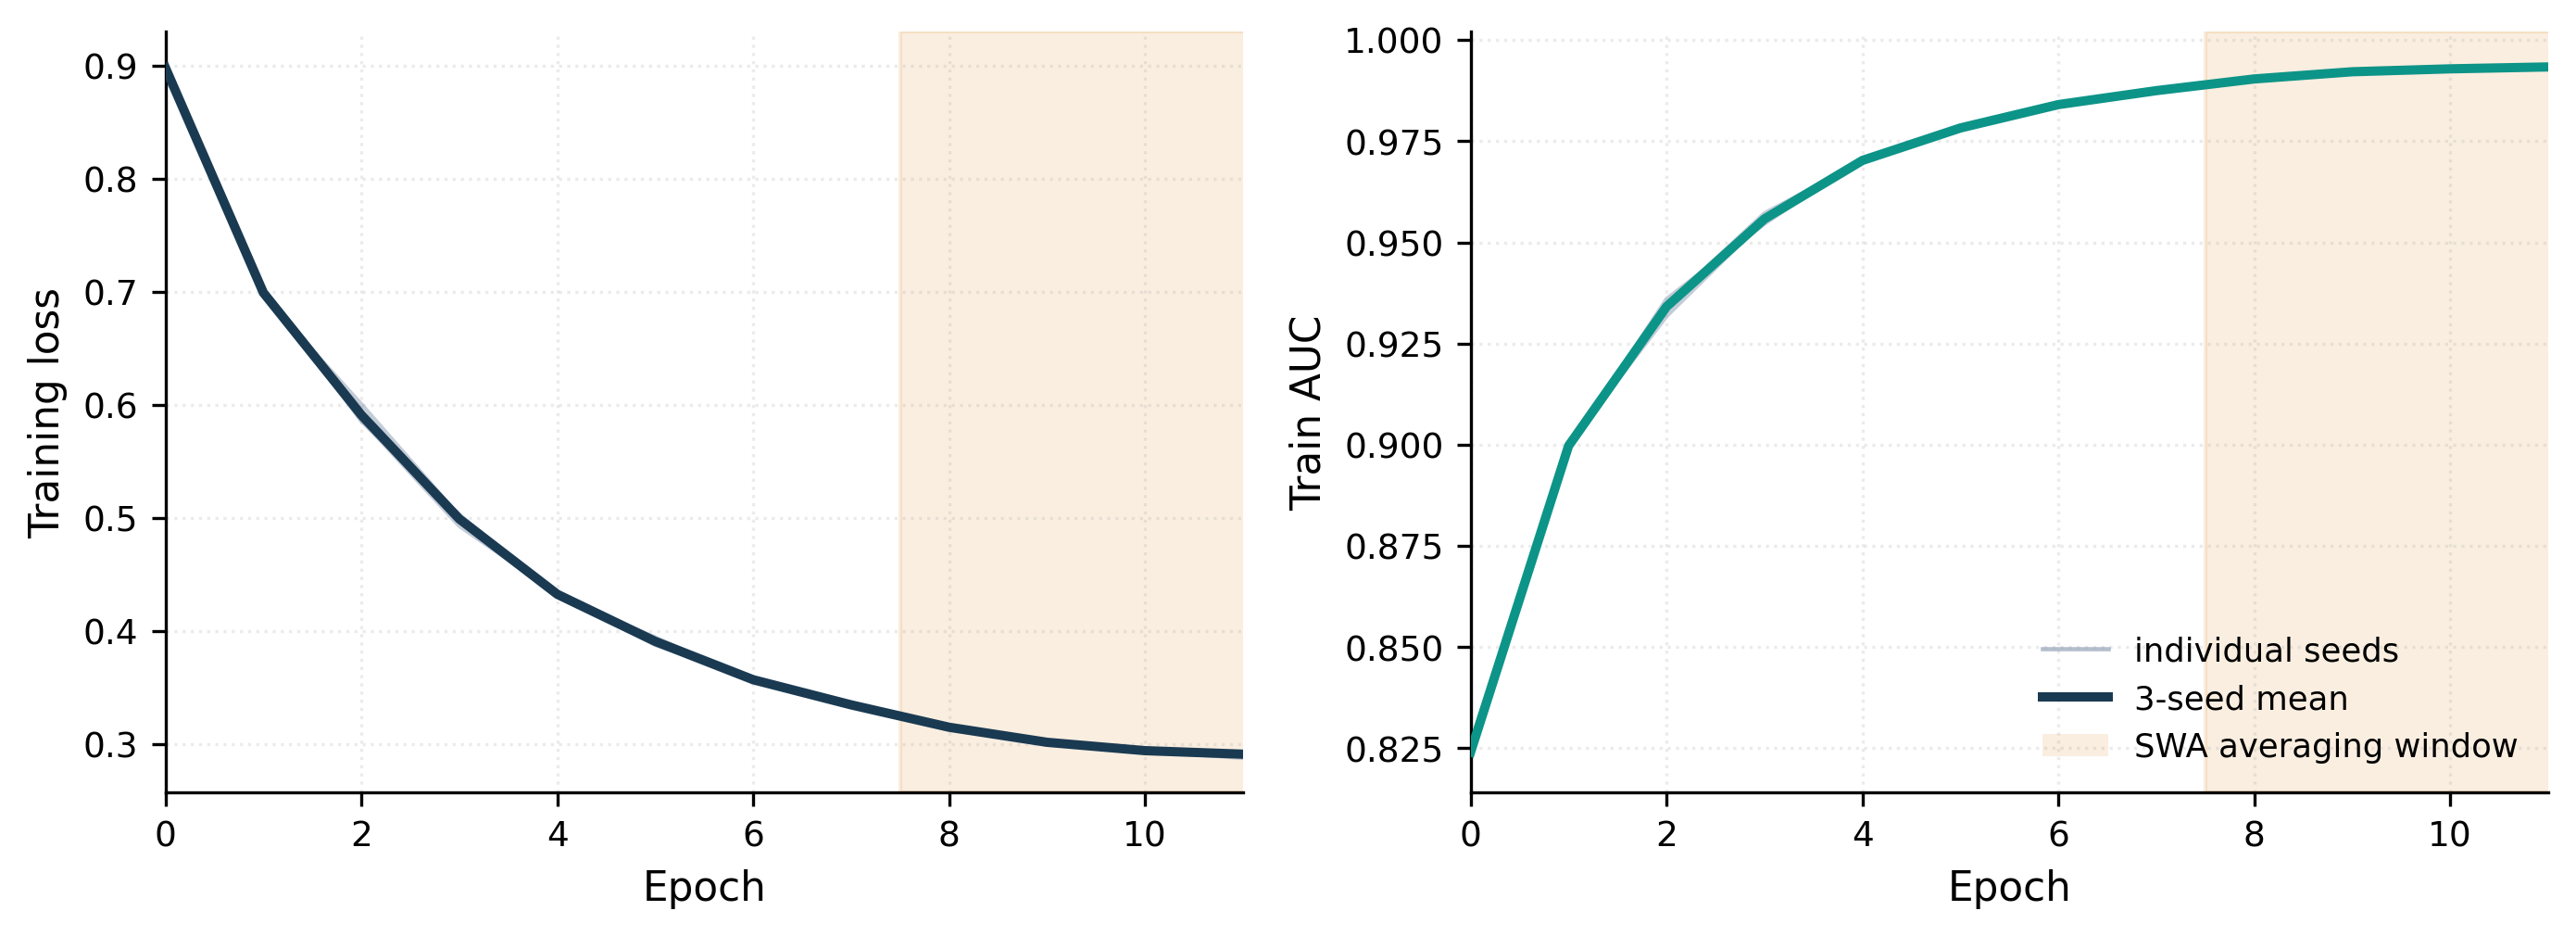
\includegraphics[width=0.95\textwidth]{learning_curves.png}
  \caption{Training curves for the final model: total training loss (left) and train AUC (right), with
  the three seeds shown individually (faint) and their mean (bold). The shaded band marks the SWA epochs
  over which weights are averaged; train AUC converges to $\approx\!0.993$ across all three seeds.}
  \label{fig:curves}
\end{figure}

\section{What did not work}

The negative results were as informative as the wins; each one revealed something about the data.

\subsection{Cross-modal self-supervised pre-training}

I tried cross-modal contrastive pre-training: an InfoNCE objective that pulls a cell's paired BF and FL
views together and pushes non-matching pairs apart, then fine-tuning for classification. It produced the
\emph{best cross-validation score} of the whole project (AUC $\approx0.866$) and then \emph{collapsed} on
the leaderboard to $\approx0.57$, essentially chance. The diagnosis is the patient shortcut: with one
patient per cell, a cell's two views always share a patient while non-matching pairs usually do not, so
the contrastive task is solvable by recognising the patient rather than the cell content. The objective
converged almost immediately, a tell-tale sign that it had found the shortcut. This failure is precisely
why the final recipe is built to suppress patient identity (AdaBN, test-set normalisation, the MIL term,
and excluding pseudo cells from the per-patient loss).

\subsection{Alternative fusion and augmentation choices}

An alternative to late fusion is intermediate co-attention fusion of the two modalities, a design
favoured in some multimodal-microscopy work. I tested two variants in that spirit: modality-specific
fluorescence augmentation and an early (input-level) fusion alternative to my late-fusion design. Both
\emph{regressed} on this dataset ($-0.036$ and $-0.031$ respectively). Design choices motivated by other
acquisition setups did not transfer to a $12$-patient, patient-disjoint regime, a reminder that reported
gains are conditional on their data.

\subsection{Stacking unvalidated changes}

One submission bundled four changes at once; it regressed and left no way to attribute the loss to any
single change. After that I adopted a strict one-or-two-changes-per-submission discipline, which is what
made the noise-floor analysis and the clean attribution in Table~\ref{tab:progression} possible.

\subsection{Ensembling across recipes}

Blending \emph{different} recipes (cross-recipe averaging, and a decorrelated feature-level GBM) never
beat the stronger member: the wide performance gaps meant the weaker model only added noise. The only
ensembling that helped was \emph{within-recipe seed averaging}, i.e.\ the three-seed mean used for the
final submission.

\section{Lessons}
\label{sec:lessons}

\begin{enumerate}
  \item \textbf{Higher CV $\neq$ higher LB on patient-grouped data.} The best CV score in the project came
        from the model that scored worst on the leaderboard. Validation must group by patient, and even
        then a held-out estimate from one or two patients is too noisy to trust.
  \item \textbf{On small $N$, dataset size beats regularisation.} Textbook regularisers added $+0.011$;
        growing the effective training set with soft pseudo-labels added $+0.042$, roughly
        $3.5\times$ larger. Capacity and regularisation were second-order next to the amount of
        supervision.
  \item \textbf{Seed variance is large; measure a noise floor.} Run-to-run AUC varied by up to
        $\sim\!0.03$ from the seed alone, so I treated any change below that as noise and averaged seeds
        for stability.
  \item \textbf{Negative results are part of the method.} The SSL collapse identified the patient
        shortcut; the failed transfer cautioned against borrowing tricks across setups; the bad stack
        enforced disciplined experimentation. The final recipe is largely a response to these failures.
  \item \textbf{Change one thing at a time.} Clean attribution is worth more than the occasional lucky
        multi-change jump.
\end{enumerate}

\section{Limitations}

Two caveats bound the headline number. First, the method is \emph{transductive}: although the test
\emph{labels} are never used, the test \emph{inputs} are consumed in three places --- AdaBN, test-set
stain normalisation, and distillation on the teacher's predictions over the full test set --- so
$0.8236$ measures performance on inputs the model was explicitly adapted to, and inductive
generalisation to a fresh patient cohort is untested. Second, every AUC reported here is on the
\emph{public} leaderboard split, which was also used for model selection across many submissions; the
public numbers are therefore an optimistic estimate of held-out performance, and the private split, not
reported here, is the unbiased measure.

\section{Conclusion}

On a $12$-patient, patient-disjoint microscopy task, the most effective strategy was not a bigger or more
exotic network but a small, shift-aware EfficientNet-B0 whose \emph{effective} training set was enlarged
with the test images via soft-target distillation. This lifted the public-leaderboard AUC from $0.7455$
to $0.8236$, a cumulative $+0.078$; the soft-distillation step alone contributed the largest single gain
($+0.042$, roughly four standard errors above the seed noise). The approaches that failed, namely cross-modal
self-supervision, same-domain transfer, stacked edits, and cross-recipe ensembling, shaped the final
recipe more than any single success.

\paragraph{Data and code availability.} The dataset is the \emph{Multimodal Cancer-Cell Classification
Challenge 2026} Kaggle competition and is not redistributed here. The training notebooks and the code
that generates every figure in this report are available at
\url{https://github.com/rafallex/multimodal-microscopy-distillation}.

\bibliographystyle{abbrvnat}
\bibliography{references}

\end{document}
